\chapter{The Lemonade}

Morrel was, in fact, very happy. M. Noirtier had just sent for him, and
he was in such haste to know the reason of his doing so that he had not
stopped to take a cab, placing infinitely more dependence on his own
two legs than on the four legs of a cab-horse. He had therefore set off
at a furious rate from the Rue Meslay, and was hastening with rapid
strides in the direction of the Faubourg Saint-Honoré.

Morrel advanced with a firm, manly tread, and poor Barrois followed him
as he best might. Morrel was only thirty-one, Barrois was sixty years
of age; Morrel was deeply in love, and Barrois was dying with heat and
exertion. These two men, thus opposed in age and interests, resembled
two parts of a triangle, presenting the extremes of separation, yet
nevertheless possessing their point of union. This point of union was
Noirtier, and it was he who had just sent for Morrel, with the request
that the latter would lose no time in coming to him—a command which
Morrel obeyed to the letter, to the great discomfiture of Barrois. On
arriving at the house, Morrel was not even out of breath, for love
lends wings to our desires; but Barrois, who had long forgotten what it
was to love, was sorely fatigued by the expedition he had been
constrained to use.

The old servant introduced Morrel by a private entrance, closed the
door of the study, and soon the rustling of a dress announced the
arrival of Valentine. She looked marvellously beautiful in her deep
mourning dress, and Morrel experienced such intense delight in gazing
upon her that he felt as if he could almost have dispensed with the
conversation of her grandfather.

But the easy-chair of the old man was heard rolling along the floor,
and he soon made his appearance in the room. Noirtier acknowledged by a
look of extreme kindness and benevolence the thanks which Morrel
lavished on him for his timely intervention on behalf of Valentine and
himself—an intervention which had saved them from despair. Morrel then
cast on the invalid an interrogative look as to the new favor which he
designed to bestow on him. Valentine was sitting at a little distance
from them, timidly awaiting the moment when she should be obliged to
speak. Noirtier fixed his eyes on her.

“Am I to say what you told me?” asked Valentine. Noirtier made a sign
that she was to do so.

“Monsieur Morrel,” said Valentine to the young man, who was regarding
her with the most intense interest, “my grandfather, M. Noirtier, had a
thousand things to say, which he told me three days ago; and now, he
has sent for you, that I may repeat them to you. I will repeat them,
then; and since he has chosen me as his interpreter, I will be faithful
to the trust, and will not alter a word of his intentions.”

“Oh, I am listening with the greatest impatience,” replied the young
man; “speak, I beg of you.”

Valentine cast down her eyes; this was a good omen for Morrel, for he
knew that nothing but happiness could have the power of thus overcoming
Valentine.

“My grandfather intends leaving this house,” said she, “and Barrois is
looking out for suitable apartments for him in another.”

“But you, Mademoiselle de Villefort,—you, who are necessary to M.
Noirtier’s happiness——”

“I?” interrupted Valentine; “I shall not leave my grandfather,—that is
an understood thing between us. My apartment will be close to his. Now,
M. de Villefort must either give his consent to this plan or his
refusal; in the first case, I shall leave directly, and in the second,
I shall wait till I am of age, which will be in about ten months. Then
I shall be free, I shall have an independent fortune, and”—

“And what?” demanded Morrel.

“And with my grandfather’s consent I shall fulfil the promise which I
have made you.”

Valentine pronounced these last few words in such a low tone, that
nothing but Morrel’s intense interest in what she was saying could have
enabled him to hear them.

“Have I not explained your wishes, grandpapa?” said Valentine,
addressing Noirtier.

“Yes,” looked the old man.

“Once under my grandfather’s roof, M. Morrel can visit me in the
presence of my good and worthy protector, if we still feel that the
union we contemplated will be likely to insure our future comfort and
happiness; in that case I shall expect M. Morrel to come and claim me
at my own hands. But, alas, I have heard it said that hearts inflamed
by obstacles to their desire grew cold in time of security; I trust we
shall never find it so in our experience!”

“Oh,” cried Morrel, almost tempted to throw himself on his knees before
Noirtier and Valentine, and to adore them as two superior beings, “what
have I ever done in my life to merit such unbounded happiness?”

“Until that time,” continued the young girl in a calm and
self-possessed tone of voice, “we will conform to circumstances, and be
guided by the wishes of our friends, so long as those wishes do not
tend finally to separate us; in a word, and I repeat it, because it
expresses all I wish to convey,—we will wait.”

“And I swear to make all the sacrifices which this word imposes, sir,”
said Morrel, “not only with resignation, but with cheerfulness.”

“Therefore,” continued Valentine, looking playfully at Maximilian, “no
more inconsiderate actions—no more rash projects; for you surely would
not wish to compromise one who from this day regards herself as
destined, honorably and happily, to bear your name?”

Morrel looked obedience to her commands. Noirtier regarded the lovers
with a look of ineffable tenderness, while Barrois, who had remained in
the room in the character of a man privileged to know everything that
passed, smiled on the youthful couple as he wiped the perspiration from
his bald forehead.

“How hot you look, my good Barrois,” said Valentine.

“Ah, I have been running very fast, mademoiselle, but I must do M.
Morrel the justice to say that he ran still faster.”

Noirtier directed their attention to a waiter, on which was placed a
decanter containing lemonade and a glass. The decanter was nearly full,
with the exception of a little, which had been already drunk by M.
Noirtier.

“Come, Barrois,” said the young girl, “take some of this lemonade; I
see you are coveting a good draught of it.”

“The fact is, mademoiselle,” said Barrois, “I am dying with thirst, and
since you are so kind as to offer it me, I cannot say I should at all
object to drinking your health in a glass of it.”

“Take some, then, and come back immediately.”

Barrois took away the waiter, and hardly was he outside the door, which
in his haste he forgot to shut, than they saw him throw back his head
and empty to the very dregs the glass which Valentine had filled.
Valentine and Morrel were exchanging their adieux in the presence of
Noirtier when a ring was heard at the door-bell. It was the signal of a
visit. Valentine looked at her watch.

“It is past noon,” said she, “and today is Saturday; I dare say it is
the doctor, grandpapa.”

Noirtier looked his conviction that she was right in her supposition.

“He will come in here, and M. Morrel had better go,—do you not think
so, grandpapa?”

“Yes,” signed the old man.

“Barrois,” cried Valentine, “Barrois!”

“I am coming, mademoiselle,” replied he.

“Barrois will open the door for you,” said Valentine, addressing
Morrel. “And now remember one thing, Monsieur Officer, that my
grandfather commands you not to take any rash or ill-advised step which
would be likely to compromise our happiness.”

\begin{figure}[ht]
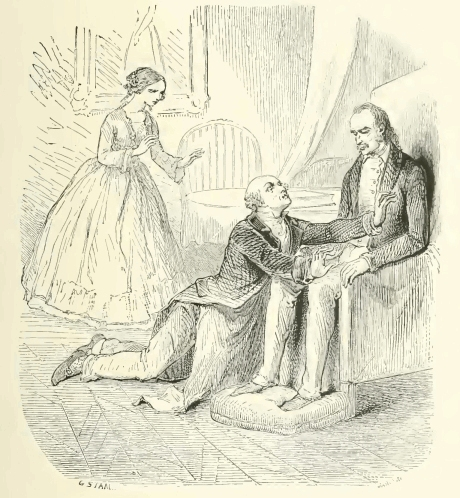
\includegraphics[width=\textwidth]{40108m.jpg}
\end{figure}

“I promised him to wait,” replied Morrel; “and I will wait.”

At this moment Barrois entered. “Who rang?” asked Valentine.

“Doctor d’Avrigny,” said Barrois, staggering as if he would fall.

“What is the matter, Barrois?” said Valentine. The old man did not
answer, but looked at his master with wild staring eyes, while with his
cramped hand he grasped a piece of furniture to enable him to stand
upright.

“He is going to fall!” cried Morrel.

The rigors which had attacked Barrois gradually increased, the features
of the face became quite altered, and the convulsive movement of the
muscles appeared to indicate the approach of a most serious nervous
disorder. Noirtier, seeing Barrois in this pitiable condition, showed
by his looks all the various emotions of sorrow and sympathy which can
animate the heart of man. Barrois made some steps towards his master.

“Ah, sir,” said he, “tell me what is the matter with me. I am
suffering—I cannot see. A thousand fiery darts are piercing my brain.
Ah, don’t touch me, pray don’t.”

By this time his haggard eyes had the appearance of being ready to
start from their sockets; his head fell back, and the lower extremities
of the body began to stiffen. Valentine uttered a cry of horror; Morrel
took her in his arms, as if to defend her from some unknown danger.

“M. d’Avrigny, M. d’Avrigny,” cried she, in a stifled voice. “Help,
help!”

Barrois turned round and with a great effort stumbled a few steps, then
fell at the feet of Noirtier, and resting his hand on the knee of the
invalid, exclaimed:

“My master, my good master!”

At this moment M. de Villefort, attracted by the noise, appeared on the
threshold. Morrel relaxed his hold of Valentine, and retreating to a
distant corner of the room remained half hidden behind a curtain. Pale
as if he had been gazing on a serpent, he fixed his terrified eye on
the agonized sufferer.

Noirtier, burning with impatience and terror, was in despair at his
utter inability to help his old domestic, whom he regarded more in the
light of a friend than a servant. One might by the fearful swelling of
the veins of his forehead and the contraction of the muscles round the
eye, trace the terrible conflict which was going on between the living
energetic mind and the inanimate and helpless body.

Barrois, his features convulsed, his eyes suffused with blood, and his
head thrown back, was lying at full length, beating the floor with his
hands, while his legs had become so stiff, that they looked as if they
would break rather than bend. A slight appearance of foam was visible
around the mouth, and he breathed painfully, and with extreme
difficulty.

Villefort seemed stupefied with astonishment, and remained gazing
intently on the scene before him without uttering a word. He had not
seen Morrel. After a moment of dumb contemplation, during which his
face became pale and his hair seemed to stand on end, he sprang towards
the door, crying out:

“Doctor, doctor! come instantly, pray come!”

“Madame, madame!” cried Valentine, calling her step-mother, and running
upstairs to meet her; “come quick, quick!—and bring your bottle of
smelling-salts with you.”

“What is the matter?” said Madame de Villefort in a harsh and
constrained tone.

“Oh! come! come!”

“But where is the doctor?” exclaimed Villefort; “where is he?”

Madame de Villefort now deliberately descended the staircase. In one
hand she held her handkerchief, with which she appeared to be wiping
her face, and in the other a bottle of English smelling-salts. Her
first look on entering the room was at Noirtier, whose face,
independent of the emotion which such a scene could not fail of
producing, proclaimed him to be in possession of his usual health; her
second glance was at the dying man. She turned pale, and her eye passed
quickly from the servant and rested on the master.

“In the name of heaven, madame,” said Villefort, “where is the doctor?
He was with you just now. You see this is a fit of apoplexy, and he
might be saved if he could but be bled!”

“Has he eaten anything lately?” asked Madame de Villefort, eluding her
husband’s question.

“Madame,” replied Valentine, “he has not even breakfasted. He has been
running very fast on an errand with which my grandfather charged him,
and when he returned, took nothing but a glass of lemonade.”

“Ah,” said Madame de Villefort, “why did he not take wine? Lemonade was
a very bad thing for him.”

“Grandpapa’s bottle of lemonade was standing just by his side; poor
Barrois was very thirsty, and was thankful to drink anything he could
find.”

Madame de Villefort started. Noirtier looked at her with a glance of
the most profound scrutiny.

“He has such a short neck,” said she.

“Madame,” said Villefort, “I ask where is M. d’Avrigny? In God’s name
answer me!”

“He is with Edward, who is not quite well,” replied Madame de
Villefort, no longer being able to avoid answering.

Villefort rushed upstairs to fetch him.

“Take this,” said Madame de Villefort, giving her smelling-bottle to
Valentine. “They will, no doubt, bleed him; therefore I will retire,
for I cannot endure the sight of blood;” and she followed her husband
upstairs. Morrel now emerged from his hiding-place, where he had
remained quite unperceived, so great had been the general confusion.

“Go away as quick as you can, Maximilian,” said Valentine, “and stay
till I send for you. Go.”

Morrel looked towards Noirtier for permission to retire. The old man,
who had preserved all his usual coolness, made a sign to him to do so.
The young man pressed Valentine’s hand to his lips, and then left the
house by a back staircase.

At the same moment that he quitted the room, Villefort and the doctor
entered by an opposite door. Barrois was now showing signs of returning
consciousness. The crisis seemed past, a low moaning was heard, and he
raised himself on one knee. D’Avrigny and Villefort laid him on a
couch.

“What do you prescribe, doctor?” demanded Villefort.

“Give me some water and ether. You have some in the house, have you
not?”

“Yes.”

“Send for some oil of turpentine and tartar emetic.”

Villefort immediately despatched a messenger. “And now let everyone
retire.”

“Must I go too?” asked Valentine timidly.

“Yes, mademoiselle, you especially,” replied the doctor abruptly.

Valentine looked at M. d’Avrigny with astonishment, kissed her
grandfather on the forehead, and left the room. The doctor closed the
door after her with a gloomy air.

“Look, look, doctor,” said Villefort, “he is quite coming round again;
I really do not think, after all, it is anything of consequence.”

M. d’Avrigny answered by a melancholy smile.

“How do you feel, Barrois?” asked he.

“A little better, sir.”

“Will you drink some of this ether and water?”

“I will try; but don’t touch me.”

“Why not?”

“Because I feel that if you were only to touch me with the tip of your
finger the fit would return.”

“Drink.”

Barrois took the glass, and, raising it to his purple lips, took about
half of the liquid offered him.

“Where do you suffer?” asked the doctor.

“Everywhere. I feel cramps over my whole body.”

“Do you find any dazzling sensation before the eyes?”

“Yes.”

“Any noise in the ears?”

“Frightful.”

\begin{figure}[ht]
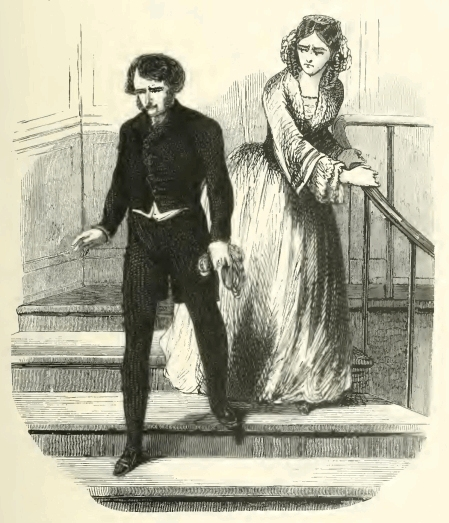
\includegraphics[width=\textwidth]{40112m.jpg}
\end{figure}

“When did you first feel that?”

“Just now.”

“Suddenly?”

“Yes, like a clap of thunder.”

“Did you feel nothing of it yesterday or the day before?”

“Nothing.”

“No drowsiness?”

“None.”

“What have you eaten today?”

“I have eaten nothing; I only drank a glass of my master’s
lemonade—that’s all.” And Barrois turned towards Noirtier, who,
immovably fixed in his armchair, was contemplating this terrible scene
without allowing a word or a movement to escape him.

“Where is this lemonade?” asked the doctor eagerly.

“Downstairs in the decanter.”

“Whereabouts downstairs?”

“In the kitchen.”

“Shall I go and fetch it, doctor?” inquired Villefort.

“No, stay here and try to make Barrois drink the rest of this glass of
ether and water. I will go myself and fetch the lemonade.”

D’Avrigny bounded towards the door, flew down the back staircase, and
almost knocked down Madame de Villefort, in his haste, who was herself
going down to the kitchen. She cried out, but d’Avrigny paid no
attention to her; possessed with but one idea, he cleared the last four
steps with a bound, and rushed into the kitchen, where he saw the
decanter about three parts empty still standing on the waiter, where it
had been left. He darted upon it as an eagle would seize upon its prey.
Panting with loss of breath, he returned to the room he had just left.
Madame de Villefort was slowly ascending the steps which led to her
room.

“Is this the decanter you spoke of?” asked d’Avrigny.

“Yes, doctor.”

“Is this the same lemonade of which you partook?”

“I believe so.”

“What did it taste like?”

“It had a bitter taste.”

The doctor poured some drops of the lemonade into the palm of his hand,
put his lips to it, and after having rinsed his mouth as a man does
when he is tasting wine, he spat the liquor into the fireplace.

“It is no doubt the same,” said he. “Did you drink some too, M.
Noirtier?”

“Yes.”

“And did you also discover a bitter taste?”

“Yes.”

“Oh, doctor,” cried Barrois, “the fit is coming on again. Oh, do
something for me.” The doctor flew to his patient.

“That emetic, Villefort—see if it is coming.”

Villefort sprang into the passage, exclaiming, “The emetic! the
emetic!—is it come yet?” No one answered. The most profound terror
reigned throughout the house.

“If I had anything by means of which I could inflate the lungs,” said
d’Avrigny, looking around him, “perhaps I might prevent suffocation.
But there is nothing which would do!—nothing!”

\begin{figure}[ht]
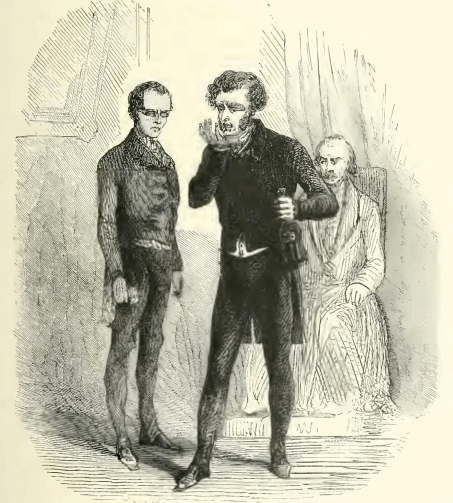
\includegraphics[width=\textwidth]{40114m.jpg}
\end{figure}

“Oh, sir,” cried Barrois, “are you going to let me die without help?
Oh, I am dying! Oh, save me!”

“A pen, a pen!” said the doctor. There was one lying on the table; he
endeavored to introduce it into the mouth of the patient, who, in the
midst of his convulsions, was making vain attempts to vomit; but the
jaws were so clenched that the pen could not pass them. This second
attack was much more violent than the first, and he had slipped from
the couch to the ground, where he was writhing in agony. The doctor
left him in this paroxysm, knowing that he could do nothing to
alleviate it, and, going up to Noirtier, said abruptly:

“How do you find yourself?—well?”

“Yes.”

“Have you any weight on the chest; or does your stomach feel light and
comfortable—eh?”

“Yes.”

“Then you feel pretty much as you generally do after you have had the
dose which I am accustomed to give you every Sunday?”

“Yes.”

“Did Barrois make your lemonade?”

“Yes.”

“Was it you who asked him to drink some of it?”

“No.”

“Was it M. de Villefort?”

“No.”

“Madame?”

“No.”

“It was your granddaughter, then, was it not?”

“Yes.”

A groan from Barrois, accompanied by a yawn which seemed to crack the
very jawbones, attracted the attention of M. d’Avrigny; he left M.
Noirtier, and returned to the sick man.

“Barrois,” said the doctor, “can you speak?” Barrois muttered a few
unintelligible words. “Try and make an effort to do so, my good man.”
said d’Avrigny. Barrois reopened his bloodshot eyes.

“Who made the lemonade?”

“I did.”

“Did you bring it to your master directly it was made?”

“No.”

“You left it somewhere, then, in the meantime?”

“Yes; I left it in the pantry, because I was called away.”

“Who brought it into this room, then?”

“Mademoiselle Valentine.” D’Avrigny struck his forehead with his hand.

“Gracious heaven,” exclaimed he.

“Doctor, doctor!” cried Barrois, who felt another fit coming.

“Will they never bring that emetic?” asked the doctor.

“Here is a glass with one already prepared,” said Villefort, entering
the room.

“Who prepared it?”

“The chemist who came here with me.”

\begin{figure}[ht]
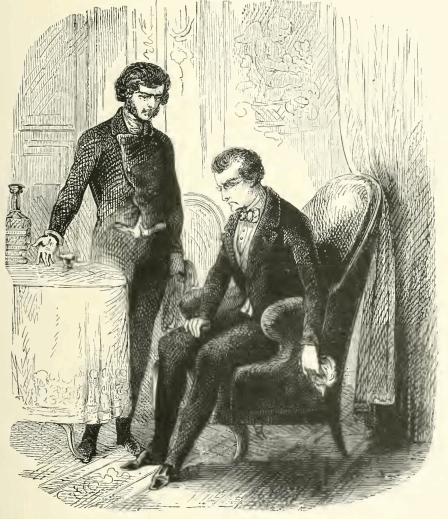
\includegraphics[width=\textwidth]{40116m.jpg}
\end{figure}

“Drink it,” said the doctor to Barrois.

“Impossible, doctor; it is too late; my throat is closing up. I am
choking! Oh, my heart! Ah, my head!—Oh, what agony!—Shall I suffer like
this long?”

“No, no, friend,” replied the doctor, “you will soon cease to suffer.”

“Ah, I understand you,” said the unhappy man. “My God, have mercy upon
me!” and, uttering a fearful cry, Barrois fell back as if he had been
struck by lightning. D’Avrigny put his hand to his heart, and placed a
glass before his lips.

“Well?” said Villefort.

“Go to the kitchen and get me some syrup of violets.”

Villefort went immediately.

“Do not be alarmed, M. Noirtier,” said d’Avrigny; “I am going to take
my patient into the next room to bleed him; this sort of attack is very
frightful to witness.”

And taking Barrois under the arms, he dragged him into an adjoining
room; but almost immediately he returned to fetch the lemonade.
Noirtier closed his right eye.

“You want Valentine, do you not? I will tell them to send her to you.”

Villefort returned, and d’Avrigny met him in the passage.

“Well, how is he now?” asked he.

“Come in here,” said d’Avrigny, and he took him into the chamber where
the sick man lay.

“Is he still in a fit?” said the procureur.

“He is dead.”

Villefort drew back a few steps, and, clasping his hands, exclaimed,
with real amazement and sympathy, “Dead?—and so soon too!”

“Yes, it is very soon,” said the doctor, looking at the corpse before
him; “but that ought not to astonish you; Monsieur and Madame de
Saint-Méran died as soon. People die very suddenly in your house, M. de
Villefort.”

“What?” cried the magistrate, with an accent of horror and
consternation, “are you still harping on that terrible idea?”

“Still, sir; and I shall always do so,” replied d’Avrigny, “for it has
never for one instant ceased to retain possession of my mind; and that
you may be quite sure I am not mistaken this time, listen well to what
I am going to say, M. de Villefort.”

The magistrate trembled convulsively.

“There is a poison which destroys life almost without leaving any
perceptible traces. I know it well; I have studied it in all its forms
and in the effects which it produces. I recognized the presence of this
poison in the case of poor Barrois as well as in that of Madame de
Saint-Méran. There is a way of detecting its presence. It restores the
blue color of litmus-paper reddened by an acid, and it turns syrup of
violets green. We have no litmus-paper, but, see, here they come with
the syrup of violets.”

The doctor was right; steps were heard in the passage. M. d’Avrigny
opened the door, and took from the hands of the chambermaid a cup which
contained two or three spoonfuls of the syrup, he then carefully closed
the door.

“Look,” said he to the procureur, whose heart beat so loudly that it
might almost be heard, “here is in this cup some syrup of violets, and
this decanter contains the remainder of the lemonade of which M.
Noirtier and Barrois partook. If the lemonade be pure and inoffensive,
the syrup will retain its color; if, on the contrary, the lemonade be
drugged with poison, the syrup will become green. Look closely!”

The doctor then slowly poured some drops of the lemonade from the
decanter into the cup, and in an instant a light cloudy sediment began
to form at the bottom of the cup; this sediment first took a blue
shade, then from the color of sapphire it passed to that of opal, and
from opal to emerald. Arrived at this last hue, it changed no more. The
result of the experiment left no doubt whatever on the mind.

“The unfortunate Barrois has been poisoned,” said d’Avrigny, “and I
will maintain this assertion before God and man.”

Villefort said nothing, but he clasped his hands, opened his haggard
eyes, and, overcome with his emotion, sank into a chair.
